\documentclass[12pt, a4paper]{article}
\usepackage[utf8]{inputenc}

\usepackage{graphicx}
\usepackage[T2A]{fontenc}
\usepackage{geometry}
\usepackage{array}
\usepackage{graphicx}
\usepackage{setspace}
\usepackage{siunitx}
\usepackage{caption}

\geometry{
    a4paper,
    left=30mm,
    right=15mm,
    top=20mm,
    bottom=20mm
}
\graphicspath{ {images/} }
\captionsetup[figure]{
    labelsep=period,    % Точка после номера
    justification=centering
}

\renewcommand{\figurename}{Рисунок}


\begin{document}
\begin{titlepage}
\begin{center}
\small
\underline{
\begin{minipage}{0.2\textwidth}
    \centering
    
\includegraphics[width=3cm]{BMSTU logo}
\end{minipage}
\hfill
\begin{minipage}{0.8\textwidth}
    \begin{center}
    
    \textbf{Министерство науки и высшего образования Российской Федерации\\
    Федеральное государственное бюджетное образовательное учреждение высшего образования «Московский государственный технический университет имени Н.Э. Баумана национальный исследовательский университет» \\
    (МГТУ им. Н.Э. Баумана)}
\end{center}
\end{minipage}

}

    \vspace{7cm}
    \Large
\textbf{Лабораторная работа Э-112}\\
"Исследование характеристик источника постоянного тока"\\
\vspace{5cm}
\normalsize
    \begin{tabular}{p{8cm}p{6cm}}
        \textbf{Студент группы ИУ1-31Б} & \hrulefill \\
        & «\underline{\hspace{1.5cm}}»\underline{\hspace{2.5cm}}2025 г. \\
        & \\
        \textbf{Преподаватель} & \hrulefill \\
        & «\underline{\hspace{1.5cm}}»\underline{\hspace{2.5cm}}2025 г. \\
    \end{tabular}
\vfill{\Large{Москва, 2025}}
\end{center}
\end{titlepage}

\textbf{Цель работы} - исследование характеристик источника постоянного тока, определение его ЭДС, внутреннего сопротивления, а также оптимального сопротивления нагрузки

\addtocounter{section}{1}
\section*{Конспект}
\subsection{Экспреиментальное оборудование, приборы и принадлежности}

\begin{figure}[ht]
    \centering{
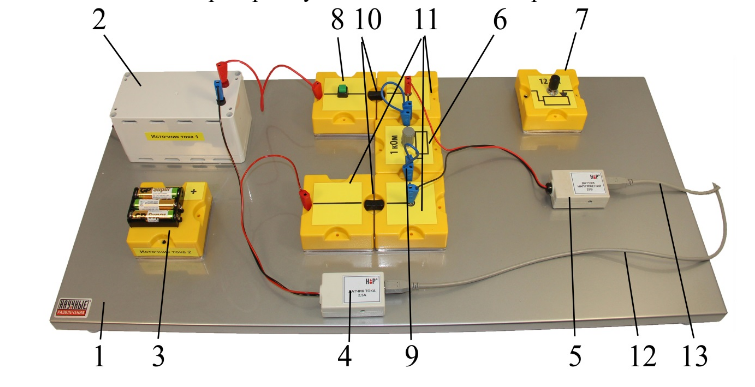
\includegraphics[width=\textwidth]{laboratory plate}
\caption{Лабораторная установка}
    }
\end{figure}
    На металлическом стенде 1, установлены: источник тока высокоомный 2, источник тока низкоомный 3 (батарейный блок), датчик тока 4, датчик напряжения 5, переменный резистор 6 (1 кОм) и переменный резистор 7 (12 Ом). Соединение цепи нагрузки с источником постоянного тока осуществляется на короткое время при включении кнопочного выключателя 8. Коммутация элементов схемы осуществляется проводами с наконечниками 9, соединителями 10 и соединительными элементами 11. Подключение датчиков к компьютеру осуществляется с помощью USB-кабелей 12 и 13. \\ 

    Также к приборам и принодлежностям относится компьютер с программным обеспечением для регистрации и обработки данных.\\

\subsection{Теоритическая часть}
\subsubsection{Электрический ток}
\hspace*{\parindent}\textbf{Электрический ток} - всякое упорядоченное движение электрических зарядов. \\

    Линии вдоль которых движутся зараяженные частицы, называются линиями тока. За направление электрического тока принимается направление движения положительных электрических зараядов. Но в действительности электрический ток в металических проводниках создается движением отрицательно зараженных электронов.\\

    \textbf{Конвекционный ток} - упорядоченное движение электрических зарядов, возникающее из-за перемещения заряжкнного тела в пространстве. \\

    \textbf{Ток в вакууме} - направленное, упорядоченное движение микроскопических зарядов независимо от макрокопических тел. \\

    \textbf{Ток проводимости} - упорядоченное направленное движение заряженных частиц в макроскопическом теле под действием электрического поля. \\

    Условия появления электричекого тока
    \begin{enumerate}
        \item Наличие свободных зарядов, которые могут свободно перемещаться.
        \item Наличие в данной среде электрического поля, энергия которого затрачивалась бы на перемещение этих частиц.
    \end{enumerate}
    
    Для того чтобы в цепи длительное время существовал ток необходимо устройство, в котором некоторый вид энергии преобразовывается в энергию электрического поля. Такое устройство называют \textbf{источником электродвижущей силы} или \textbf{источником тока}\\


    \hspace*{\parindent}\textbf{Сила тока} - скалярная величина численно равная электрическому заряду прошедшему через попереченое сечение проводника за единицу времени. \\

    \begin{equation}
        \label{eq:elctricForce}
    I = \frac{dq}{dt}
    \end{equation}
    В уравнении \ref{eq:elctricForce} dq - электрический заряд проходящий черех попереченое сечение проводника за время dt. \\

    Если сила тока не изменяется со временем, то такой ток называется постоянным. В этом случае сила тока: \\

    \begin{equation}
        \label{eq:constelctricForce}
    I = \frac{q}{t}
    \end{equation}

    В уравнении \ref{eq:constelctricForce} q - электрический заряд проходящий черех попереченое сечение проводника за время t. \\

    Единица силы тока в системе СИ - ампер (А). Он определяется на основании электромагнитного взаимодействия двух параллельных прямолинейных постоянных токов. \\

    Для характеристики распределения электрического тока по сечению проводника вводится понятие вектора плотности тока $\vec{j}$, его направленние совпадает с направлением тока в проводнике, а модуль равен силе тока в расчете на единицу площади сечения проводника, перпендикулярной к линиям тока. \\

    \begin{equation}
        \label{eq:densityVector}
        j=\frac{dI}{dS}
    \end{equation}

    В уравнении \ref{eq:densityVector} dI - сила тока проходящая через элементарную площадку dS, расположенную перпендикулярно к вектору $\vec{j}$. Единица измерения в системе СИ - $\text{А}/\text{м}^2$. \\

    Из уравнения \ref{eq:densityVector} следует, что полная сила тока в проводнике \\

    \begin{equation}
        \label{eq:fullElectricForce}
        I = \int\limits_{S}^{} {jdS}
    \end{equation}

    Если площадка dS не перпендикулярна $\vec{j}$ берется составляющая $j_n = jcosa$ перпендикулярная к ней. Поэтому для постоянного тока 

    \begin{equation}
        \label{eq:constFullElectricForce}
        I = jS
    \end{equation}

    В цепи постоянного тока, состоящей из проводников с переменной площадью сечения, плотности токов в различных  сечениях $S_1$ и $S_2$ обратно пропорциональны площадям этих сечений. \\


    \begin{equation}
        \label{eq:fracOfDensityVectors}
        \frac{j_1}{j_2}=\frac{S_2}{S_1}
    \end{equation}

    Электроны проводимости в металле, ионы в электролите, ионы и электроны в газе, т.е. все заряженные частицы, содержащиеся в различных телах, совершают хаотическое (тепловое) движение. \\
    
    Электрическое поле $\vec{E}$  в веществе сообщает всем свободным заряженным частицам дополнительную скорость упорядоченного движения, которое обуславливает ток. Средняя скорость этого движения в твердых веществах и жидкостях составляет около $10^-3$-$10^-5\text{м}/\text{с}$. Однако эта скорость не имеет ничего общего со скоростью распространения тока в проводниках которая равна скорости света в веществе откружающем его. \\
    
    \begin{equation}
        \label{eq:speedOfElectricity}
        v = \frac{c}{\sqrt{\epsilon{}\mu{}}}
    \end{equation}

    где с - скорость света в вакууме, $\epsilon$ - диэлектрическая проницаемость среды, $\mu$ - магнитная проницаемость среды.\\

    Выделим внутри проводника площадку dS перпендикулярную $\vec{\mu}$. Построим на этой площадке цилиндр с высотой равной $\mu dt$ (Рисунока \ref{fig:cilinder}). Тогда число частиц, которые пройдут через эту площадку за время dt, будет равно числу частиц заключенных в этом цилиндре.
    \begin{figure}[ht]
        \centering
            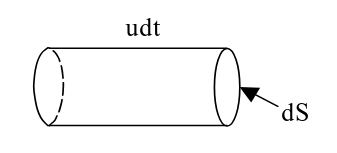
\includegraphics{cilinder}
            \caption{}
            \label{fig:cilinder}
    \end{figure}

    Если e - заряд носителя тока, n - концентрация заряженных частиц, то число частиц внутри цилиндра равно $nudtds$, а заряд переносимый через площадку dS будет $q = en\mu dtdS$. \\

    Отсюда величина плотности тока \\

    \begin{equation}
        \label{eq:densityVectorModule}
        j = \frac{dq}{dtdS} = enu
    \end{equation}

    Так как e и n скалярные величины, а скорость $\vec{u}$

    \begin{equation}
        \label{eq:densityVectorEq}
        \vec{j} = en\vec{u}
    \end{equation}

    \subsubsection{Элетктродвижущая сила.}

    Если в проводнике создать электричекое поле и не принять мер к его поддепжанию, то перемещение зарядов приведет к его исчезновению, и как следствие прекращению тока. Для поддержания тока необходимо постоянно переносить заряды от конца провожника с меньшим потенциалом $\phi_2$ к понцу проводника с большим потенциалом $\phi_1$ (\ref{fig:potentials}).

    \begin{figure}[ht]
        \centering
            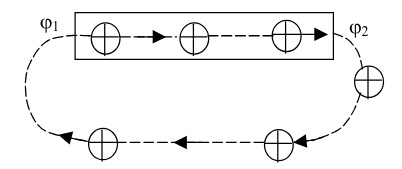
\includegraphics{potentials}
            \caption{}
            \label{fig:potentials}
    \end{figure}

    Такое перемещение возможно только с помощью сил неэлектростатического происхождения, называемх сторонними. Такие силы можно охарактеризовать их работой. \\

    \textbf{Электродвижущая сила (ЭДС), действующая в электрической цепи или на её участке, численно равна работе совершаемой сторонними силами при перемещении по электрической цепи или по её участку единичного положительного заряда.} \\

    \begin{equation}
        \label{eq:electricityMoveForce}
        \varepsilon = \frac{A_\text{ст}}{q}
    \end{equation}

    $\varepsilon$ измеряется в вольтах.\\

    Сторонняя сила\\
    \begin{equation}
        \label{eq:sideForce}
        \vec{F} = q\vec{E^\text{*}}
    \end{equation} 

    Векторную величину $\vec{E^\text{*}}$ называют напряженностью  поля сторонниз сил. Работу таких сил над зарядом q на всём протяжении замкнутой цепи можно представить следующим образом \\

    \begin{equation}
        \label{eq:sideForceWork}
        A = \oint{A_\text{ст}d\vec{I}} = \oint{q\vec{E^\text{*}}d\vec{I}}
    \end{equation} 

    Отсюда ЭДС действующая в цепи равна 

    \begin{equation}
        \label{eq:curcuitElctricForce}
        \varepsilon= \oint{q\vec{E^\text{*}}d\vec{I}}
    \end{equation} 

    Электродвижущая сила на участке 1-2, равна \\

    \begin{equation}
        \label{eq:curcuitPartElctricForce}
        \varepsilon= \int\limits_{1}^{2}{q\vec{E^\text{*}}d\vec{I}}
    \end{equation} 

    Кроме сторонних сил на заряд действуют силы электростатического поля $\vec{F_\text{э}}=q\vec{E}$. Следовательно результирующая сила, действующая в каждой точке цепи на заряд q, равна 

    \begin{equation}
        \label{eq:resForce}
        \vec{F} = \vec{F_\text{э}} + \vec{F_\text{ст}} = q(\vec{E} + \vec{E^\text{*}}).
    \end{equation} 

    Работа совершаемая этой силой над зарядом q на участке 1-2, даётся выражением \\

    \begin{equation}
        \label{eq:resWork}
        A = q\int\limits_{1}^{2}\vec{E}d\vec{I} +  q\int\limits_{1}^{2}\vec{E^\text{*}}d\vec{I} = q\varepsilon_\text{1,2} + q(\phi_1 - \phi_2).
    \end{equation} 

    \textbf{Величина, числено равная работе, совершаемой электростатическими и сторонними силами при перемещении единичного положительного заряда, называется падением напряжения или напряжением U на данном участке цепи}

    \begin{equation}
        \label{eq:voltage}
        U_\text{1,2} = \phi_1 - \phi_2 + \varepsilon_\text{1,2}.
    \end{equation} 

    При отсутствии сторонних сил напряжение совпадает с разностьью потенциалов. \\ 

    \begin{equation}
        \label{eq:voltageWithoutSideForce}
        U_\text{1,2} = \phi_1 - \phi_2.
    \end{equation} 
\end{document}